\documentclass[acmtog]{acmart}
\usepackage{graphicx}
\usepackage{subfigure}
\usepackage{natbib}
\usepackage{listings}
\usepackage{bm}
\usepackage{amsmath}

\definecolor{blve}{rgb}{0.3372549 , 0.61176471, 0.83921569}
\definecolor{gr33n}{rgb}{0.29019608, 0.7372549, 0.64705882}
\makeatletter
\lst@InstallKeywords k{class}{classstyle}\slshape{classstyle}{}ld
\makeatother
% \lstset{language=C++,
% 	basicstyle=\ttfamily,
% 	keywordstyle=\color{blve}\ttfamily,
% 	stringstyle=\color{red}\ttfamily,
% 	commentstyle=\color{magenta}\ttfamily,
% 	morecomment=[l][\color{magenta}]{\#},
% 	classstyle = \bfseries\color{gr33n}, 
% 	tabsize=2
% }
\lstset{ %
backgroundcolor=\color{white},   % choose the background color
basicstyle=\footnotesize\ttfamily,        % size of fonts used for the code
columns=fullflexible,
breaklines=true,                 % automatic line breaking only at whitespace
captionpos=b,                    % sets the caption-position to bottom
tabsize=4,
commentstyle=\color{mygreen},    % comment style
escapeinside={\%*}{*)},          % if you want to add LaTeX within your code
keywordstyle=\color{blue},       % keyword style
stringstyle=\color{mymauve}\ttfamily,     % string literal style
frame=single,
rulesepcolor=\color{red!20!green!20!blue!20},
% identifierstyle=\color{red},
language=c++,
}
\lstset{basicstyle=\ttfamily}

% Title portion
\title{Assignment 5:\\ {Animation with Cloth Simulation}} 

\author{Name:\quad Entropy-Fighter\\ student number:\ 2020533
\\email:\quad xxxx@shanghaitech.edu.cn}

% Document starts
\begin{document}
\maketitle

\vspace*{2 ex}

\section{Introduction}
In this homework, I do the following things.
\begin{itemize}
	\item Force computation with Hooke's law (30 pts)
	\item Structural, shear, and bending springs (40 pts)
	\item Fix the location of two mesh points to stop the cloth falling down (10 pts)
	\item Real-time and stable animation (10 pts)
	\item (bonus)Apply external forces to the cloth to simulate the behavior of wind (5 pts)
	\item (bonus)Add a sphere or cube obstacle to simulate a piece of cloth falling on a sphere or a cube with collision handling (10 pts)
	\item (bonus)Drag a mesh point to move the cloth with mouse in real-time (15 pts)
\end{itemize}
\section{Implementation Details}
\subsection{Force computation with Hooke's law}
\quad This section is implemented in the ComputeHookeForce function in the "cloth.cpp". I write this function based on the Hooke's law.
The Hooke's law is clearly shown in the tutorial's PPT below.
\begin{figure}[h]
	\centering
	{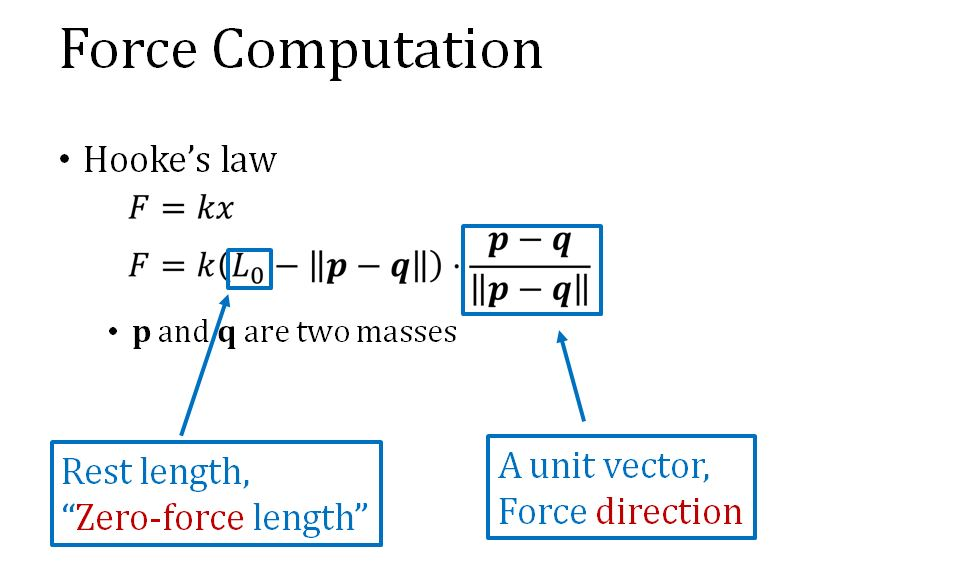
\includegraphics[width=8cm]{hook.JPG}}	
\end{figure}


Note that before we use the hooke's law to compute hooke force, we should consider some special cases and set the force to {0, 0, 0}
The code about the special cases is listed below.
\begin{lstlisting}
	if(iw_this < 0 || iw_this >= mass_dim.x || iw_that >= mass_dim.x || ih_this < 0 || ih_this >= mass_dim.y || ih_that >= mass_dim.y){
    	return {0, 0, 0};
  	}
\end{lstlisting}
\subsection{Structural, shear, and bending springs}
\quad This section is implemented in the ComputeSpringForce function in the "cloth.cpp". Firstly, let us look at the graphical examples to understand what are the 
structural, shear, and bending springs.
\begin{figure}[h]
	\centering
	{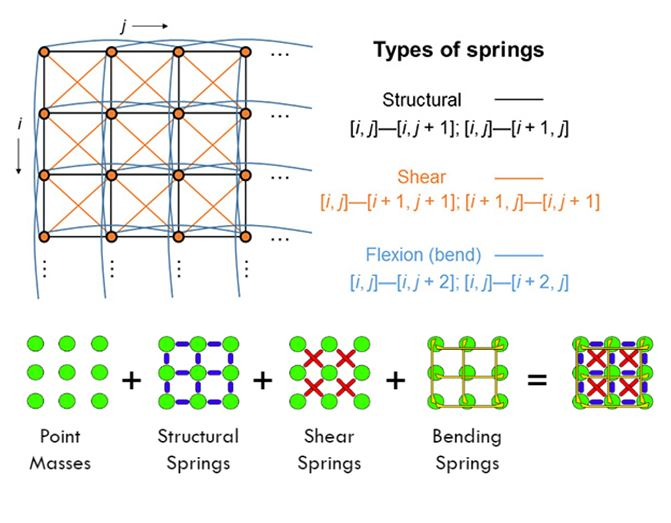
\includegraphics[width=8cm]{spring.JPG}}	
\end{figure}

THerefore, when we compute the spring force, we should consider all 3 situations. The code is shown below.
\begin{lstlisting}
	Force += ComputeHookeForce(iw, ih, iw - 1, ih, dx_local * scale[0]);
	Force += ComputeHookeForce(iw, ih, iw, ih - 1, dx_local * scale[1]);
	Force += ComputeHookeForce(iw, ih, iw + 1, ih, dx_local * scale[0]);
	Force += ComputeHookeForce(iw, ih, iw, ih + 1, dx_local * scale[1]);

	Force += ComputeHookeForce(iw, ih, iw - 2, ih, 2 * dx_local * scale[0]);
	Force += ComputeHookeForce(iw, ih, iw, ih - 2, 2 * dx_local * scale[1]);
	Force += ComputeHookeForce(iw, ih, iw + 2, ih, 2 * dx_local * scale[0]); 
	Force += ComputeHookeForce(iw, ih, iw, ih + 2, 2 * dx_local * scale[1]);

	Float hypotenuse = std::sqrt(scale[0] * scale[0] + scale[1] * scale[1]);
	Force += ComputeHookeForce(iw, ih, iw - 1, ih - 1, dx_local * hypotenuse);
	Force += ComputeHookeForce(iw, ih, iw - 1, ih + 1, dx_local * hypotenuse);
	Force += ComputeHookeForce(iw, ih, iw + 1, ih - 1, dx_local * hypotenuse);
	Force += ComputeHookeForce(iw, ih, iw + 1, ih + 1, dx_local * hypotenuse);
\end{lstlisting}
\subsection{Fix the location of two mesh points to stop the cloth falling down}
\quad This part is implemented in the ComputeAccelerations, ComputeVelocities and ComputePositions function in the "cloth.cpp".
As for the fixed points, we consider them as special cases, we should set their accelerations, velocities and positions properly. 
The pesudo code is shown below.
\begin{lstlisting}
	if(is_fixed_masses[i]) {
		world_accelerations[i] = Vec3(0.0f, 0.0f, 0.0f);
		world_velocities[i] = Vec3(0.0f, 0.0f, 0.0f);
		continue;
	}
\end{lstlisting}
\subsection{Real-time and stable animation (10 pts)}
\quad This section is implemented in the ComputeAccelerations, ComputeVelocities and ComputePositions function in the "cloth.cpp". 
As for accelerations, the formula is a = F/m - g. The code is shown below.
\begin{lstlisting}
	world_accelerations[i] = (ComputeSpringForce(iw, ih) - damping_ratio * world_velocities[i]) / mass_weight - gravity;
\end{lstlisting}
As for velocities, the formula is v = v0 + at. The code is shown below.
\begin{lstlisting}
	world_velocities[i] += world_accelerations[i] * fixed_delta_time;
\end{lstlisting}
AS for positions, the formula is s = s0 + vt
\begin{lstlisting}
	local_or_world_positions[i] += fixed_delta_time * world_velocities[i];
\end{lstlisting}
\subsection{(bonus)Apply external forces to the cloth to simulate the behavior of wind}
\quad This section is implemented in the fluid function in "cloth.cpp". This function is to add another force to simulate the wind.
The core code for constructing such a force is shown below.
\begin{lstlisting}
	return Float(0.02) * glm::dot((Vec3(0, 0, 3) - v), vertices[i].normal) * vertices[Get1DIndex(iw, ih)].normal;
\end{lstlisting}

Also, when we caculate the accelerations, we should add this new force.
\subsection{(bonus)Add a sphere or cube obstacle to simulate a piece of cloth falling on a sphere or a cube with collision handling}
\quad In this section, I add a sphere to simulate a piece of cloth falling on a sphere with collision detection. The collision detection section is implemented in the s\_intersect function in "cloth.cpp". The key 
idea is to compare r and the distance. The core code is shown below.
\begin{lstlisting}
	if(glm::length(pos - c) >= r)
		return false;
	else
		return true;
\end{lstlisting}

Note that when the cloth falls on the sphere, we should accordingly modify the acceleration, velocity and the position. 
The pesudo code for such cases is shown below.
\begin{lstlisting}
	if(s_intersect(local_or_world_positions[i]) || is_fixed_masses[i]) {
		world_accelerations[i] = Vec3(0.0f, 0.0f, 0.0f);
		world_velocities[i] = Vec3(0.0f, 0.0f, 0.0f);
		local_or_world_positions[i] = c + r * glm::normalize(local_or_world_positions[i] - c) + Float(0.04) * glm::normalize(local_or_world_positions[i] - c);
		continue;
	}
\end{lstlisting}
\quad The code for position seems a bit long. If we don't add the last term, the position will be on the sphere, which would look like weird.
\subsection{(bonus)Drag a mesh point to move the cloth with mouse in real-time}
\quad This section is implemented in the "main.cpp". In this section, I add 2 features. If we drag the cloth by left mouse, the whole clothes would move. Otherwise, if we drag the cloth by right mouse, the effect is similar to dragging the cloth by finger.
As for the first feature, my key idea is similar to my second homework's bonus(drag the control points). I use two important and useful functions, which are glReadPixels() function and glm::unProject() function. By using this 2 functions, I can get my cursor's world position on the object. When I move my mouse, I modify the 
all mass's world position to achive the moving effect.

As for the second feature, I use another way. Like homework3, I generate a ray from the camera. The generated ray will intersect the near plane. Then, I use some tricks to find the closest mass. How to change the position of the mass? I caculate the moving distance by similar triangle, then I change the position accordingly.
\section{Results}
% pictures should be in
\begin{figure}[h]
	\centering
	{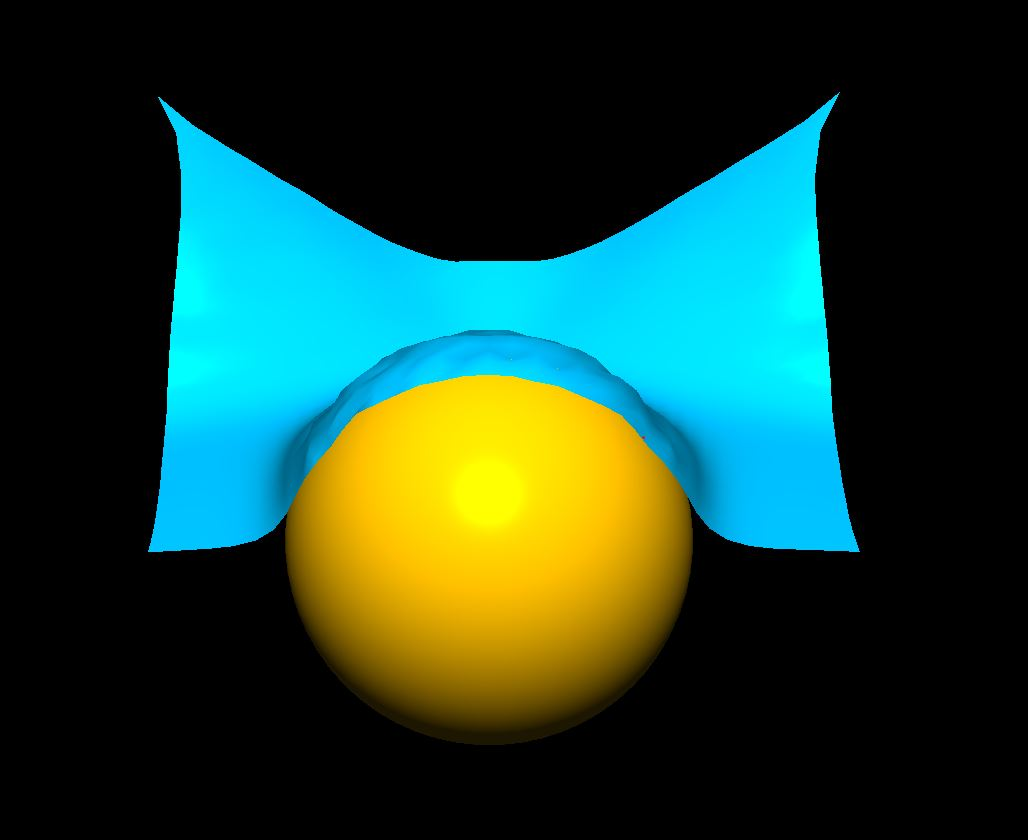
\includegraphics[width=8cm]{sphere.JPG}}	
	\caption{fall on the sphere}
\end{figure}
\begin{figure}[h]
	\centering
	{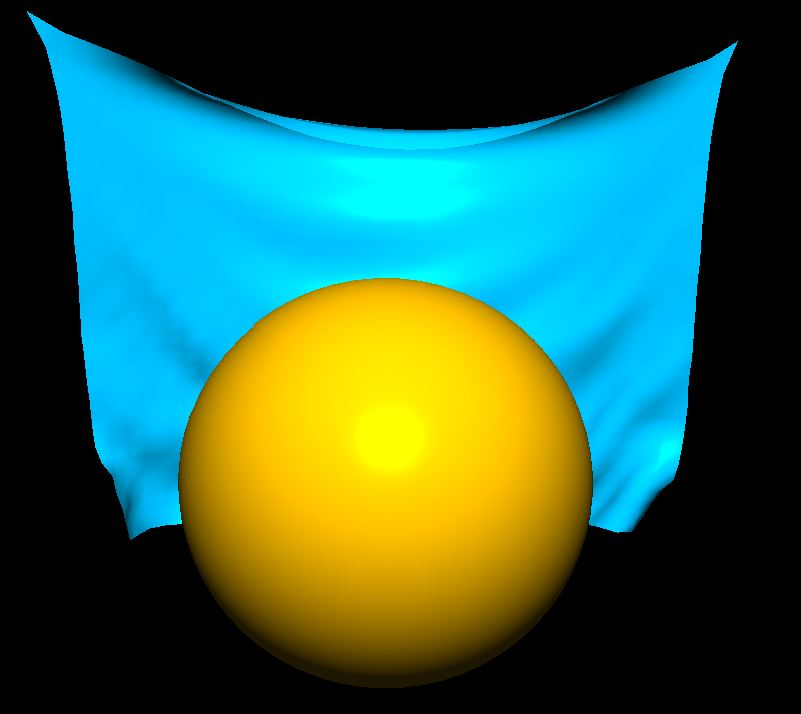
\includegraphics[width=8cm]{wind.JPG}}	
	\caption{cloth with wind}
\end{figure}
\begin{figure}[h]
	\centering
	{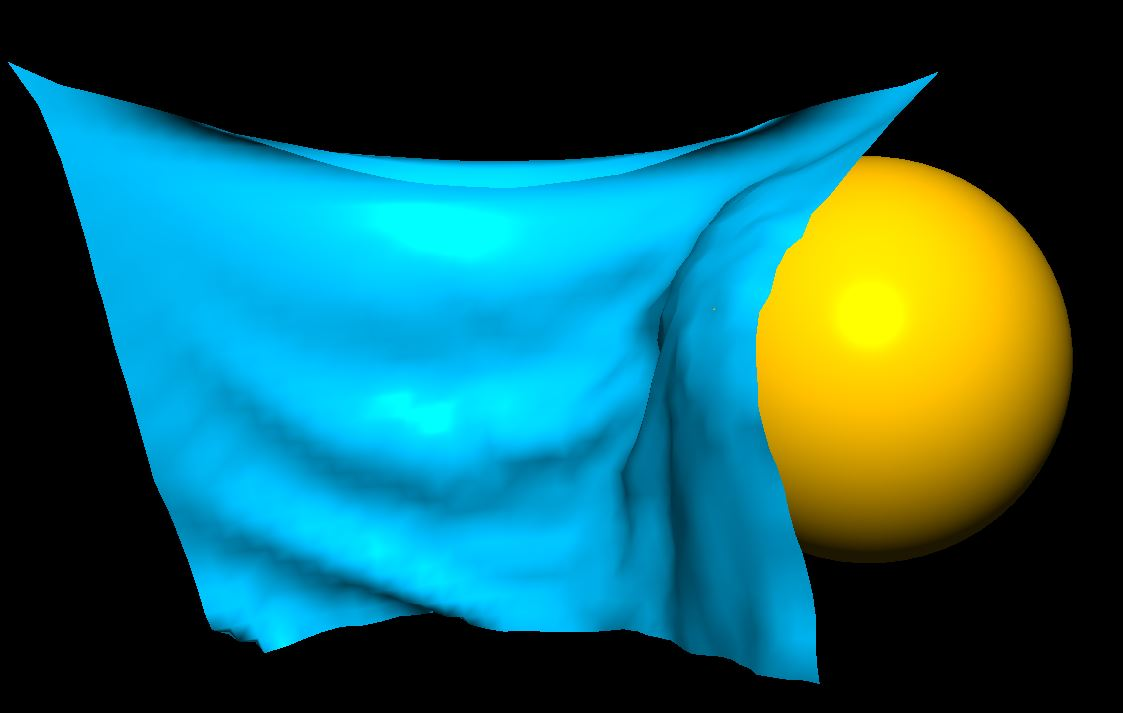
\includegraphics[width=8cm]{moveL.JPG}}
	\caption{drag with left mouse(move the whole cloth)}	
\end{figure}
\begin{figure}[h]
	\centering
	{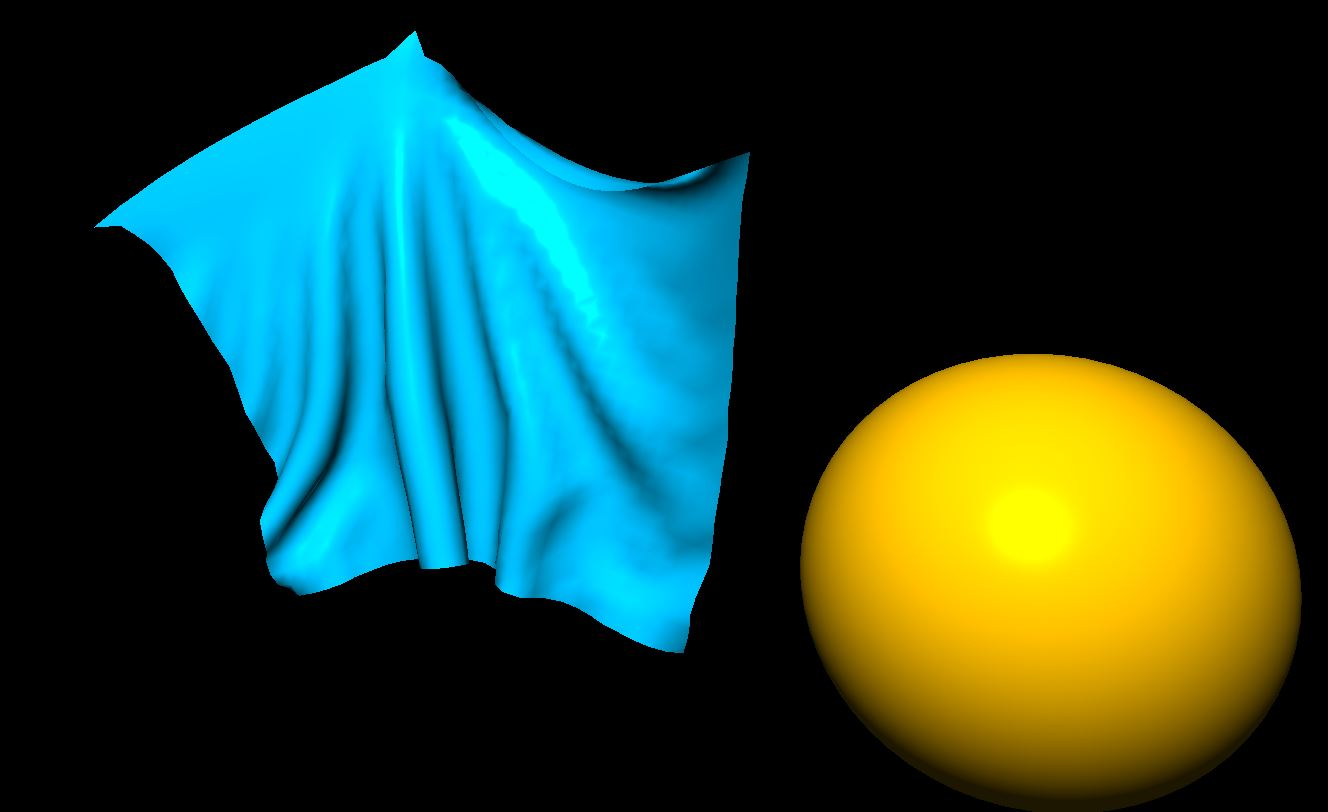
\includegraphics[width=8cm]{moveR.JPG}}
	\caption{drag with right mouse(move one point)}	
\end{figure}

\end{document}
